\section{Joint Distributions}

\begin{definition}
    The \textit{joint probability mass function} (joint PMF) of two discrete random variables \( X \) and \( Y \), denoted as \( P(X = x, Y = y) \), gives the probability that \( X \) takes on the value \( x \) and \( Y \) takes on the value \( y \). The joint PMF must satisfy the following properties:

\[
P(X = x, Y = y) \geq 0 \quad \forall x, y,
\]
\[
\sum_{x} \sum_{y} P(X = x, Y = y) = 1.
\]
\end{definition}

\begin{example}
    Consider two dice rolls \( X \) and \( Y \). The joint PMF can be represented as follows:

\[
P(X = x, Y = y) = \frac{1}{36} \quad \text{for } x, y \in \{1, 2, \ldots, 6\}.
\]

This means that each combination of dice rolls has an equal probability of \( \frac{1}{36} \).
\end{example}

\begin{definition}
    The \textit{marginal probability mass function} (marginal PMF) for a discrete random variable \( X \) can be derived from the joint PMF by summing over all possible values of the other variable \( Y \):

\[
P(X = x) = \sum_{y} P(X = x, Y = y).
\]
\end{definition}

\begin{example}
    Continuing with the dice example, the marginal PMF of \( X \) is given by:

\[
P(X = x) = \sum_{y=1}^{6} P(X = x, Y = y) = \sum_{y=1}^{6} \frac{1}{36} = \frac{6}{36} = \frac{1}{6} \quad \text{for } x \in \{1, 2, \ldots, 6\}.
\]
\end{example}

\begin{definition}
    The \textit{conditional probability mass function} (conditional PMF) describes the probability of \( X \) given that \( Y \) has occurred, denoted as \( P(X = x \mid Y = y) \). It is calculated using the joint PMF as follows:

\[
P(X = x \mid Y = y) = \frac{P(X = x, Y = y)}{P(Y = y)},
\]
provided that \( P(Y = y) > 0 \).

\end{definition}

\begin{example}
    Using our dice example, if we want to find the conditional PMF of \( X \) given \( Y = 3 \):

\[
P(X = x \mid Y = 3) = \frac{P(X = x, Y = 3)}{P(Y = 3)}.
\]

Calculating \( P(Y = 3) \):

\[
P(Y = 3) = \sum_{x=1}^{6} P(X = x, Y = 3) = \sum_{x=1}^{6} \frac{1}{36} = \frac{6}{36} = \frac{1}{6}.
\]

Thus, the conditional PMF is:

\[
P(X = x \mid Y = 3) = \frac{P(X = x, Y = 3)}{\frac{1}{6}} = P(X = x, Y = 3) \cdot 6 = \frac{6}{36} = \frac{1}{6} \quad \text{for } x \in \{1, 2, \ldots, 6\}.
\]
\end{example}

\begin{definition}
    The \textit{joint probability density function} (joint PDF) of two continuous random variables \( X \) and \( Y \) is a function \( f_{X,Y}(x,y) \) that describes the likelihood of \( X \) and \( Y \) simultaneously taking on specific values. The joint PDF must satisfy the following properties:\\

1. \( f_{X,Y}(x,y) \geq 0 \) for all \( x, y \).\\
2. The integral of the joint PDF over the entire space must equal 1:
\[
\iint_{\mathbb{R}^2} f_{X,Y}(x,y) \, dx \, dy = 1.
\]
\end{definition}

    Consider \( X \) and \( Y \) representing the height and weight of individuals in a population. The joint PDF might be expressed as:
\[
f_{X,Y}(x,y) = \frac{1}{2\pi \sigma_x \sigma_y} e^{-\frac{(x - \mu_x)^2}{2\sigma_x^2} - \frac{(y - \mu_y)^2}{2\sigma_y^2}},
\]
where \( \mu_x, \mu_y \) are the means and \( \sigma_x, \sigma_y \) are the standard deviations of the respective distributions.

\begin{definition}
    The \textit{marginal probability density function} of a random variable is obtained by integrating the joint PDF over the other variable. For example, the marginal PDF of \( X \) is given by:
\[
f_X(x) = \int_{-\infty}^{\infty} f_{X,Y}(x,y) \, dy.
\]
Similarly, the marginal PDF of \( Y \) is:
\[
f_Y(y) = \int_{-\infty}^{\infty} f_{X,Y}(x,y) \, dx.
\]
\end{definition}

Using the joint PDF example above, the marginal PDF of \( X \) can be computed as:
\[
f_X(x) = \int_{-\infty}^{\infty} f_{X,Y}(x,y) \, dy.
\]
This gives the distribution of \( X \) regardless of \( Y \).

\begin{definition}
    The \textit{conditional probability density function} describes the probability of one random variable given the value of another. The conditional PDF of \( Y \) given \( X = x \) is defined as:
\[
f_{Y|X}(y|x) = \frac{f_{X,Y}(x,y)}{f_X(x)},
\]
provided \( f_X(x) > 0 \).
\end{definition}

Using the same joint PDF, the conditional PDF of \( Y \) given \( X = x \) is:
\[
f_{Y|X}(y|x) = \frac{f_{X,Y}(x,y)}{f_X(x)}.
\]
This expresses how \( Y \) behaves when \( X \) is fixed at a certain value.\\

\begin{example}
    Let \( X \) and \( Y \) be two continuous random variables that follow a bivariate normal distribution with the following parameters:
\begin{itemize}
    \item Means: \( \mu_X = 0 \), \( \mu_Y = 0 \)
    \item Variances: \( \sigma_X^2 = 1 \), \( \sigma_Y^2 = 1 \)
    \item Covariance: \( \text{Cov}(X, Y) = \rho \) (where \( -1 < \rho < 1 \))
\end{itemize}

The joint PDF of \( X \) and \( Y \) is given by:
\begin{align*}
    f_{X,Y}(x,y) &= \frac{1}{2\pi \sigma_X \sigma_Y \sqrt{1 - \rho^2}} \\
    &\quad \times \exp\left(-\frac{1}{2(1 - \rho^2)} \left(\frac{(x - \mu_X)^2}{\sigma_X^2} + \frac{(y - \mu_Y)^2}{\sigma_Y^2} - 2\rho \frac{(x - \mu_X)(y - \mu_Y)}{\sigma_X \sigma_Y}\right)\right).
    \end{align*}
    
The conditional PDF of \( Y \) given \( X = x_0 \) is derived from the joint PDF:
\[
f_{Y|X}(y|x_0) = \frac{f_{X,Y}(x_0, y)}{f_X(x_0)}.
\]

The formula for the conditional PDF of a bivariate normal distribution is:
\[
f_{Y|X}(y|x_0) = \frac{1}{\sqrt{2\pi \sigma_Y^2 (1 - \rho^2)}} \exp\left(-\frac{1}{2(1 - \rho^2)} \left(\frac{(y - \mu_{Y|X})^2}{\sigma_{Y|X}^2}\right)\right),
\]
where:
\begin{align*}
\mu_{Y|X} &= \mu_Y + \rho \frac{\sigma_Y}{\sigma_X}(x_0 - \mu_X), \\
\sigma_{Y|X}^2 &= \sigma_Y^2 (1 - \rho^2).
\end{align*}

Let’s take:
\begin{itemize}
    \item \( \rho = 0.5 \)
    \item \( x_0 = 1 \)
\end{itemize}

We can compute:\\
1. Mean of \( Y \) given \( X = 1 \):
   \[
   \mu_{Y|X} = 0 + 0.5 \cdot \frac{1}{1}(1 - 0) = 0.5.
   \]

2. Variance of \( Y \) given \( X = 1 \):
   \[
   \sigma_{Y|X}^2 = 1 \cdot (1 - 0.5^2) = 1 \cdot 0.75 = 0.75.
   \]

So the conditional PDF of \( Y \) given \( X = 1 \) is:
\[
f_{Y|X}(y|1) = \frac{1}{\sqrt{2\pi \cdot 0.75}} \exp\left(-\frac{(y - 0.5)^2}{2 \cdot 0.75}\right).
\]

This describes the distribution of \( Y \) when \( X \) is fixed at \( 1 \). The resulting distribution is still normal, with mean \( 0.5 \) and variance \( 0.75 \).

\end{example}

In the case of a bivariate normal distribution, the joint PDF can be visualized as a 3D surface where the height of the surface at any point \( (x, y) \) represents the density of the joint occurrence of \( X \) and \( Y \).

\begin{center}
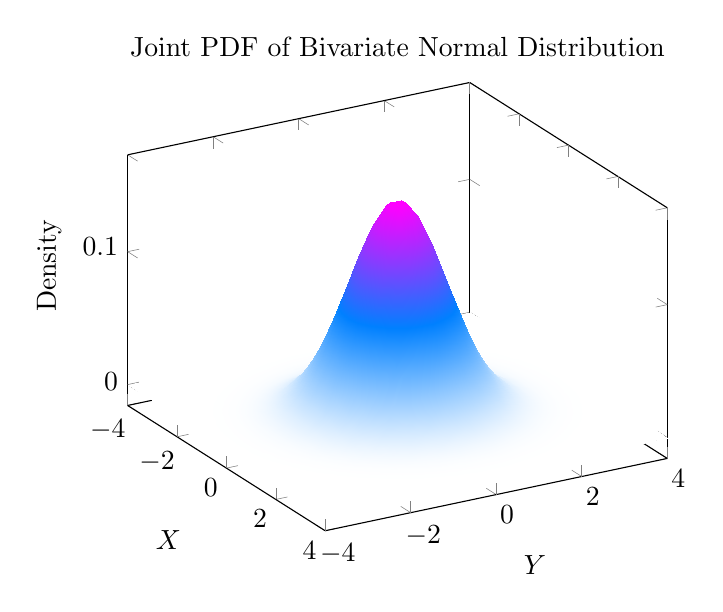
\begin{tikzpicture}
    \begin{axis}[
        xlabel={$X$},
        ylabel={$Y$},
        zlabel={Density},
        title={Joint PDF of Bivariate Normal Distribution},
        domain=-4:4,
        domain y=-4:4,
        samples=30,
        samples y=30,
        z buffer=sort,
        mesh/cols=30,
        view={60}{30},
        colormap/cool
    ]
    \addplot3[
        surf,
        shader=interp,
        samples=50,
        z buffer=sort,
        domain=-4:4,
        domain y=-4:4
    ]
    {1/(2*pi)*exp(-0.5*(x^2 + y^2))}; % Bivariate Normal PDF
    \end{axis}
\end{tikzpicture}
\end{center}

The marginal PDF can be visualized as the height of the surface obtained by fixing one variable and observing the distribution of the other. For example, the marginal PDF of \( X \) can be visualized as a 2D slice of the joint PDF along the \( X \)-axis. 
\begin{center}
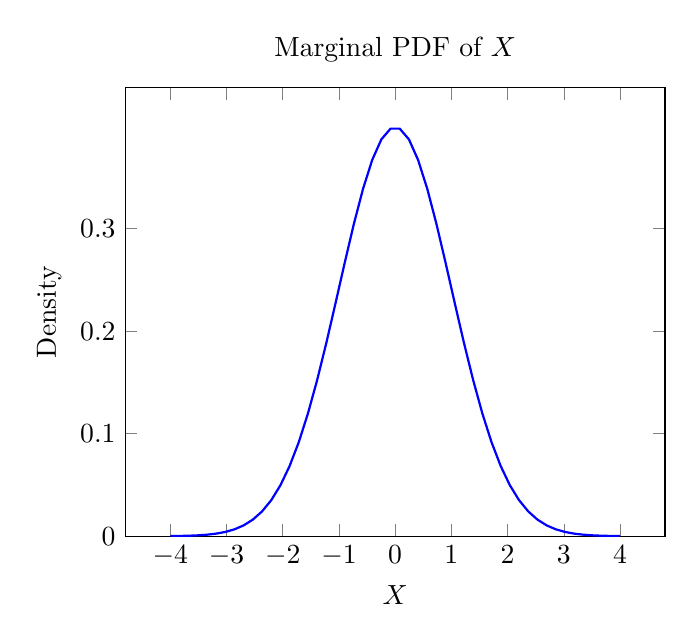
\begin{tikzpicture}
    \begin{axis}[
        xlabel={$X$},
        ylabel={Density},
        title={Marginal PDF of $X$},
        domain=-4:4,
        samples=50,
        ymin=0,
        ytick={0,0.1,0.2,0.3},
        xtick={-4,-3,-2,-1,0,1,2,3,4}
    ]
    \addplot[blue, thick] {1/sqrt(2*pi)*exp(-0.5*x^2)};
    \end{axis}
\end{tikzpicture}
\end{center}

Remember, for conditional probability, we take a vertical slice of the joint PDF corresponding to the observed value of \( X \); since the total area under this slice is \( f_X(x) \), we then divide by \( f_X(x) \) to ensure that the conditional PDF will have an area of 1.

\begin{center}
    \begin{tikzpicture}[scale=0.8]
        % 3D Normal distribution
        \begin{axis}[
            width=10cm, height=8cm,
            xlabel=$X$, ylabel=$Y$, zlabel={$f_{X,Y}(x,y)$},
            xlabel style={sloped like x axis},
            ylabel style={sloped like y axis},
            zmin=0, zmax=0.2,
            view={30}{20},
            colormap/cool
        ]
            \addplot3[
                surf,
                samples=30,
                domain=-3:3,
                y domain=-3:3,
            ] {exp(-(x^2+y^2)/2)/(2*pi)};
            
            % Vertical slice
            \addplot3[domain=-3:3, samples=30, color=red, thick] 
                ({1}, x, {exp(-(1^2+x^2)/2)/(2*pi)});
            
            % Highlight observed X value
            \draw[dashed, thick] (axis cs:1,-3,0) -- (axis cs:1,3,0);
            \node[below] at (axis cs:1,-3,0) {$x$};
        \end{axis}
        
        % Annotation for joint PDF
        \node[above] at (current axis.north east) {Joint PDF $f_{X,Y}(x,y)$};
        
        % 2D slice
        \begin{axis}[
            at={($(current axis.east)+(3cm,0)$)},
            anchor=west,
            width=6cm, height=8cm,
            xlabel=$Y$, ylabel={$f_{Y|X}(y|x)$},
            title={Conditional PDF},
            ymin=0, ymax=0.5,
        ]
            \addplot[domain=-3:3, samples=100, thick, color=red] 
                {exp(-x^2/2)/sqrt(2*pi)};
            \addplot[domain=-3:3, samples=100, dashed] 
                {0.5*exp(-x^2/2)/sqrt(2*pi)};
            \node at (axis cs:2.5,0.45) {$\frac{f_{X,Y}(x,y)}{f_X(x)}$};
            \node[color=red] at (axis cs:-2.5,0.35) {Normalized};
        \end{axis}
    \end{tikzpicture}
    \end{center}

\subsection{Independence of Random Variables}

Two random variables \( X \) and \( Y \) are said to be \textit{independent} if the occurrence of one does not affect the probability distribution of the other. This concept can be formally defined in terms of their joint and marginal probability mass functions (PMFs).

\begin{definition}
    The random variables \( X \) and \( Y \) are independent if and only if the following condition holds for all \( x \) and \( y \):

\[
P(X = x, Y = y) = P(X = x) P(Y = y).
\]

\end{definition}

This means that the joint PMF of \( X \) and \( Y \) can be expressed as the product of their marginal PMFs.

\subsubsection{Equivalent Conditions}

The independence of random variables can also be expressed in several equivalent forms:\\

1. \textbf{For all Events}: \( X \) and \( Y \) are independent if for any two events \( A \) and \( B \),
   \[
   P(A \cap B) = P(A) P(B).
   \]

2. \textbf{In terms of Expectations}: If \( X \) and \( Y \) are independent, then for any functions \( g \) and \( h \),
   \[
   E[g(X) h(Y)] = E[g(X)] E[h(Y)].
   \]

\begin{example}
    Consider two dice rolls \( X \) and \( Y \), where \( X \) represents the outcome of the first die and \( Y \) represents the outcome of the second die. Since the outcome of one die does not affect the outcome of the other, we can show their independence.\\

The joint PMF is given by:
\[
P(X = x, Y = y) = \frac{1}{36} \quad \text{for } x, y \in \{1, 2, \ldots, 6\}.
\]

The marginal PMFs are:
\[
P(X = x) = \frac{1}{6} \quad \text{and} \quad P(Y = y) = \frac{1}{6}.
\]

Verifying independence:
\[
P(X = x, Y = y) = \frac{1}{36} = P(X = x) P(Y = y) = \left(\frac{1}{6}\right)\left(\frac{1}{6}\right) = \frac{1}{36}.
\]

Thus, \( X \) and \( Y \) are independent random variables.
\end{example}

\begin{example}
    Consider two independent continuous random variables \( X \) and \( Y \) with the following PDFs:

\[
f_X(x) = \begin{cases} 
\frac{1}{2} & \text{for } 0 < x < 2 \\
0 & \text{otherwise}
\end{cases}, \quad
f_Y(y) = \begin{cases} 
\frac{1}{3} & \text{for } 0 < y < 3 \\
0 & \text{otherwise}
\end{cases}.
\]

The joint PDF of \( X \) and \( Y \) is:

\[
f_{X,Y}(x,y) = f_X(x) \cdot f_Y(y) = \begin{cases} 
\frac{1}{6} & \text{for } 0 < x < 2 \text{ and } 0 < y < 3 \\
0 & \text{otherwise}
\end{cases}.
\]

This demonstrates that \( X \) and \( Y \) are independent, as the joint PDF is indeed the product of the marginal PDFs.
\end{example}

\subsection{Covariance and Correlation}

\begin{definition}
    The covariance of two random variables \(X\) and \(Y\) is a measure of the degree to which the two variables change together. It is defined mathematically as:

\[
\text{Cov}(X, Y) = E\left[(X - E[X])(Y - E[Y])\right] = E[XY] - E[X]E[Y],
\]

where \(E[X]\) and \(E[Y]\) are the expected values (means) of \(X\) and \(Y\), respectively.
\end{definition}

\textbf{Interpretation}:

\begin{itemize}
    \item If \(\text{Cov}(X, Y) > 0\): \(X\) and \(Y\) tend to increase together.
    \item If \(\text{Cov}(X, Y) < 0\): When \(X\) increases, \(Y\) tends to decrease, and vice versa.
    \item If \(\text{Cov}(X, Y) = 0\): There is no linear relationship between \(X\) and \(Y\).
\end{itemize}

\begin{figure}[h]
    \centering
    \begin{tikzpicture}[scale=0.7]
        % Positive Correlation
        \begin{axis}[
            at={(0,0)},
            width=6cm, height=6cm,
            xlabel=$X$, ylabel=$Y$,
            title={Positive Correlation},
            xtick=\empty, ytick=\empty,
            xmin=-1, xmax=11, ymin=-1, ymax=11,
        ]
            \addplot[only marks, mark=*, mark size=1.5pt, color=blue] 
                coordinates {
                    (1,1.5) (2,2.2) (3,3.1) (4,3.8) (5,4.5)
                    (6,5.7) (7,6.4) (8,7.2) (9,8.1) (10,9.3)
                };
        \end{axis}
        
        % Negative Correlation
        \begin{axis}[
            at={(7cm,0)},
            width=6cm, height=6cm,
            xlabel=$X$, ylabel=$Y$,
            title={Negative Correlation},
            xtick=\empty, ytick=\empty,
            xmin=-1, xmax=11, ymin=-1, ymax=11,
        ]
            \addplot[only marks, mark=*, mark size=1.5pt, color=red] 
                coordinates {
                    (1,9.5) (2,8.8) (3,7.9) (4,7.2) (5,6.5)
                    (6,5.3) (7,4.6) (8,3.8) (9,2.9) (10,1.7)
                };
        \end{axis}
        
        % No Correlation
        \begin{axis}[
            at={(14cm,0)},
            width=6cm, height=6cm,
            xlabel=$X$, ylabel=$Y$,
            title={No Correlation},
            xtick=\empty, ytick=\empty,
            xmin=-1, xmax=11, ymin=-1, ymax=11,
        ]
            \addplot[only marks, mark=*, mark size=1.5pt, color=green!50!black] 
                coordinates {
                    (1,5.5) (2,3.2) (3,8.1) (4,2.8) (5,9.5)
                    (6,1.7) (7,6.4) (8,4.2) (9,7.1) (10,5.3)
                };
        \end{axis}
    \end{tikzpicture}
\end{figure}

\begin{example}
    Consider two random variables \(X\) and \(Y\) with the following joint distribution:

\[
\begin{array}{c|cccc}
X \backslash Y & 1 & 2 & 3 \\
\hline
1 & 0.1 & 0.2 & 0.1 \\
2 & 0.2 & 0.1 & 0.1 \\
3 & 0.1 & 0.1 & 0.1 \\
\end{array}
\]

First, we calculate the marginal distributions:

\[
P(X = 1) = 0.4, \quad P(X = 2) = 0.4, \quad P(X = 3) = 0.2,
\]
\[
P(Y = 1) = 0.4, \quad P(Y = 2) = 0.4, \quad P(Y = 3) = 0.2.
\]

Next, we calculate the expected values:

\[
E[X] = 1 \cdot 0.4 + 2 \cdot 0.4 + 3 \cdot 0.2 = 1.8,
\]
\[
E[Y] = 1 \cdot 0.4 + 2 \cdot 0.4 + 3 \cdot 0.2 = 1.8.
\]

Next, we calculate \(E[XY]\):

\[
E[XY] = 1\cdot1 \cdot 0.1 + 1\cdot2 \cdot 0.2 + 1\cdot3 \cdot 0.1 + 2\cdot1 \cdot 0.2 + 2\cdot2 \cdot 0.1 + 2\cdot3 \cdot 0.1 + 
\]
\[
    3\cdot1 \cdot 0.1 + 3\cdot2 \cdot 0.1 + 3\cdot3 \cdot 0.1 = 1.4.
\]

Now we calculate the covariance:

\[
\text{Cov}(X, Y) = E[XY] - E[X]E[Y] = 1.4 - (1.8 \cdot 1.8) = 1.4 - 3.24 = -1.84.
\]

This negative covariance indicates that \(X\) and \(Y\) tend to move in opposite directions.
\end{example}

\subsubsection{Properties of Covariance}

1. Symmetry: 
   \[
   \text{Cov}(X, Y) = \text{Cov}(Y, X).
   \]

2. Linearity: For any constants \(a\) and \(b\),
   \[
   \text{Cov}(aX + b, Y) = a \cdot \text{Cov}(X, Y).
   \]

3. Independence: If \(X\) and \(Y\) are independent, then:
   \[
   \text{Cov}(X, Y) = 0.
   \]

4. Variance Relation: The covariance of a random variable with itself is its variance:
   \[
   \text{Cov}(X, X) = \text{Var}(X).
   \]

\begin{definition}
    The correlation between two random variables \( X \) and \( Y \) is a measure of the strength and direction of their linear relationship. It is defined mathematically as:

\[
\rho(X, Y) = \frac{\text{Cov}(X, Y)}{\sigma_X \sigma_Y}
\]

where \( \text{Cov}(X, Y) \) is the covariance between \( X \) and \( Y \), and \( \sigma_X \) and \( \sigma_Y \) are the standard deviations of \( X \) and \( Y \), respectively. The correlation coefficient \( \rho(X, Y) \) ranges from -1 to 1.
\end{definition}

\textbf{Difference between Covariance and Correlation:}\\

Covariance provides information about the direction of the relationship but is affected by the scale of the variables. Correlation standardizes this relationship, making it easier to interpret the strength and direction of the relationship without the influence of scale.